% =====================================================================
%  FraudLens - Slide B flow : Learning and Serving (blocks 6-11)
%  Compile:  pdflatex flow_b.tex
%  PNG    :  pdftoppm -r 400 -png flow_b.pdf flow_b
% =====================================================================
\documentclass[border=5pt]{standalone}

\usepackage[T1]{fontenc}
\usepackage{amsmath}
\usepackage{tikz}
\usetikzlibrary{arrows.meta}
\hyphenpenalty=10000 \exhyphenpenalty=10000

\definecolor{hiFill}{HTML}{E6E6F7}
\definecolor{hiLine}{HTML}{2A2A8C}
\definecolor{inkCol}{HTML}{111111}

\begin{document}
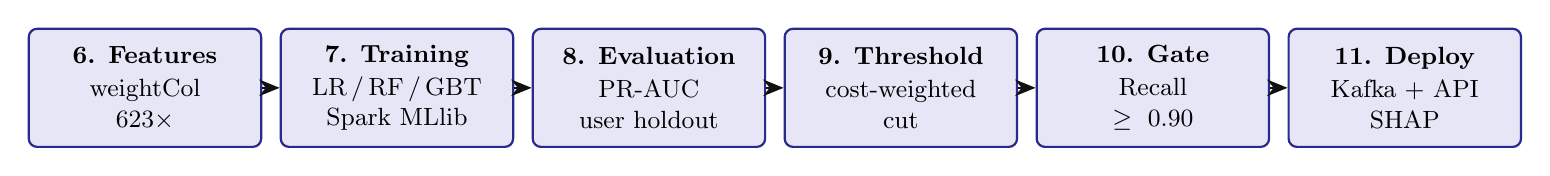
\begin{tikzpicture}[
  font=\small,
  blk/.style={
    draw=hiLine, line width=0.8pt, rounded corners=3pt,
    fill=hiFill, align=center, inner sep=5pt,
    text width=26mm, minimum height=15mm
  },
  ar/.style={-{Stealth[length=2.6mm,width=2.1mm]}, line width=0.8pt, inkCol}
]

\def\cx{32mm}

\node[blk] (b1) at (0*\cx,0) {\textbf{6. Features}\\[1pt]weightCol\\623$\times$};
\node[blk] (b2) at (1*\cx,0) {\textbf{7. Training}\\[1pt]LR\,/\,RF\,/\,GBT\\Spark MLlib};
\node[blk] (b3) at (2*\cx,0) {\textbf{8. Evaluation}\\[1pt]PR-AUC\\user holdout};
\node[blk] (b4) at (3*\cx,0) {\textbf{9. Threshold}\\[1pt]cost-weighted\\cut};
\node[blk] (b5) at (4*\cx,0) {\textbf{10. Gate}\\[1pt]Recall\\$\geq 0.90$};
\node[blk] (b6) at (5*\cx,0) {\textbf{11. Deploy}\\[1pt]Kafka + API\\SHAP};

\draw[ar] (b1) -- (b2);
\draw[ar] (b2) -- (b3);
\draw[ar] (b3) -- (b4);
\draw[ar] (b4) -- (b5);
\draw[ar] (b5) -- (b6);

\end{tikzpicture}
\end{document}
